\section{选题背景}

\begin{frame}{宏观经济和政府调控}

  \begin{itemize}
\item
政府是指导和调控经济运行的主体。国民经济的发展和政府的指导
和调控紧密相关。

\item
政府部门需要时刻把握国民经济的方方面面,要研究这些经济变量
发生变化的原因以及各种经济变量
之间的作用关系。

\item
只有这样,政府才能发现经济中存在的问题,并且给出针对性的指
导和调控手段。
  \end{itemize}
\end{frame}

\begin{frame}{把控宏观经济数据}
  \begin{itemize}
    \item
    政府需要时刻把控宏观经济指标的当前水平。
  \end{itemize}
\begin{figure}[H]
  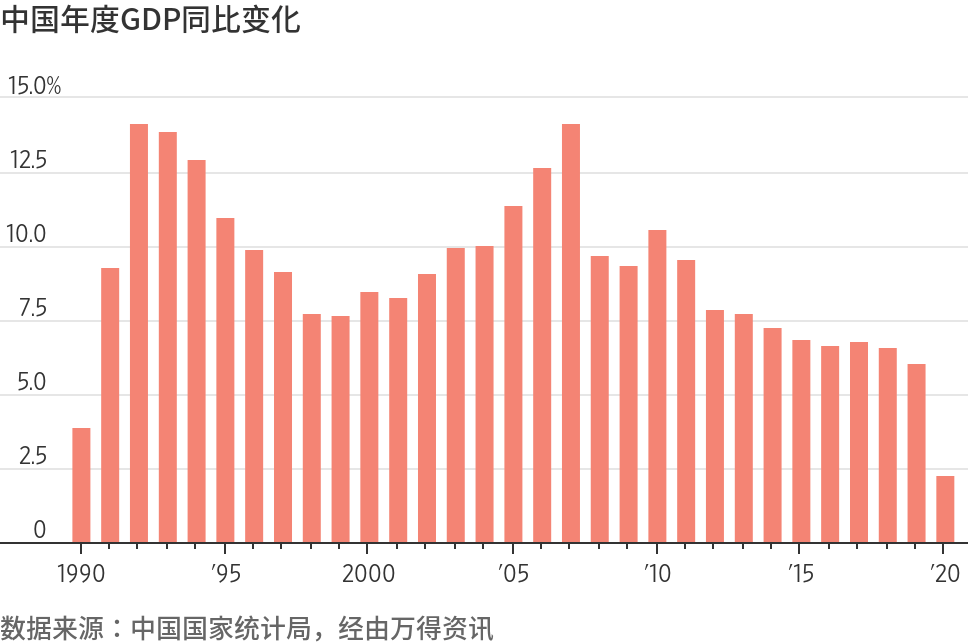
\includegraphics[width=5cm]{pics/gdp.png}
  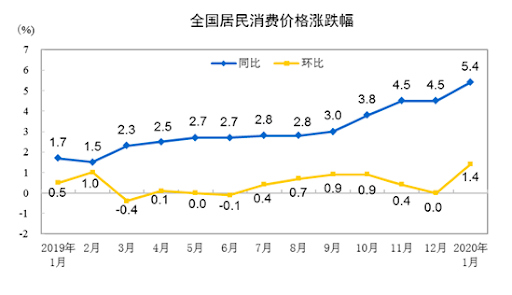
\includegraphics[width=5cm]{pics/price.png}
\end{figure}
\end{frame}

\begin{frame}{宏观经济现状分析}
  \begin{itemize}
    \item
    通过对当前宏观经济指标数据的综合分析,观察当前宏观经济
    的运行状况,便于行使见机行事的宏观经济政策。
  \end{itemize}
\begin{figure}[H]
  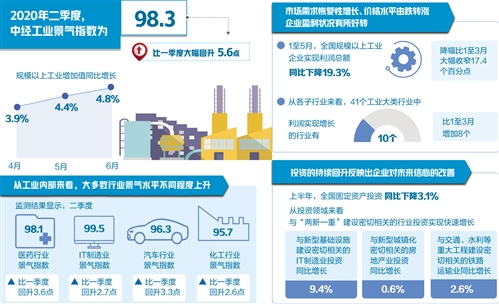
\includegraphics[width=8cm]{pics/macro-demo.jpeg}
\end{figure}
\end{frame}

\begin{frame}{宏观经济预测}
  \begin{itemize}
    \item
    政府和研究机构常常对重要经济指标做出预测
  \end{itemize}
\begin{figure}[H]
  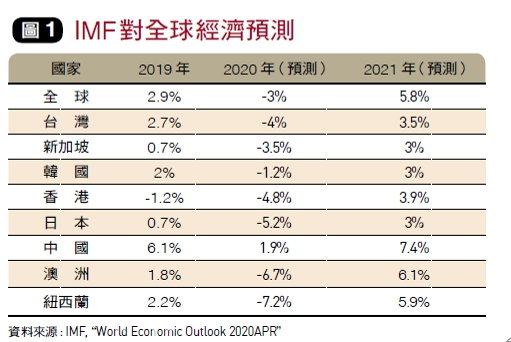
\includegraphics[width=8cm]{pics/predict-demo.jpeg}
\end{figure}
\end{frame}

\begin{frame}{宏观经济预测}

\begin{figure}[H]
  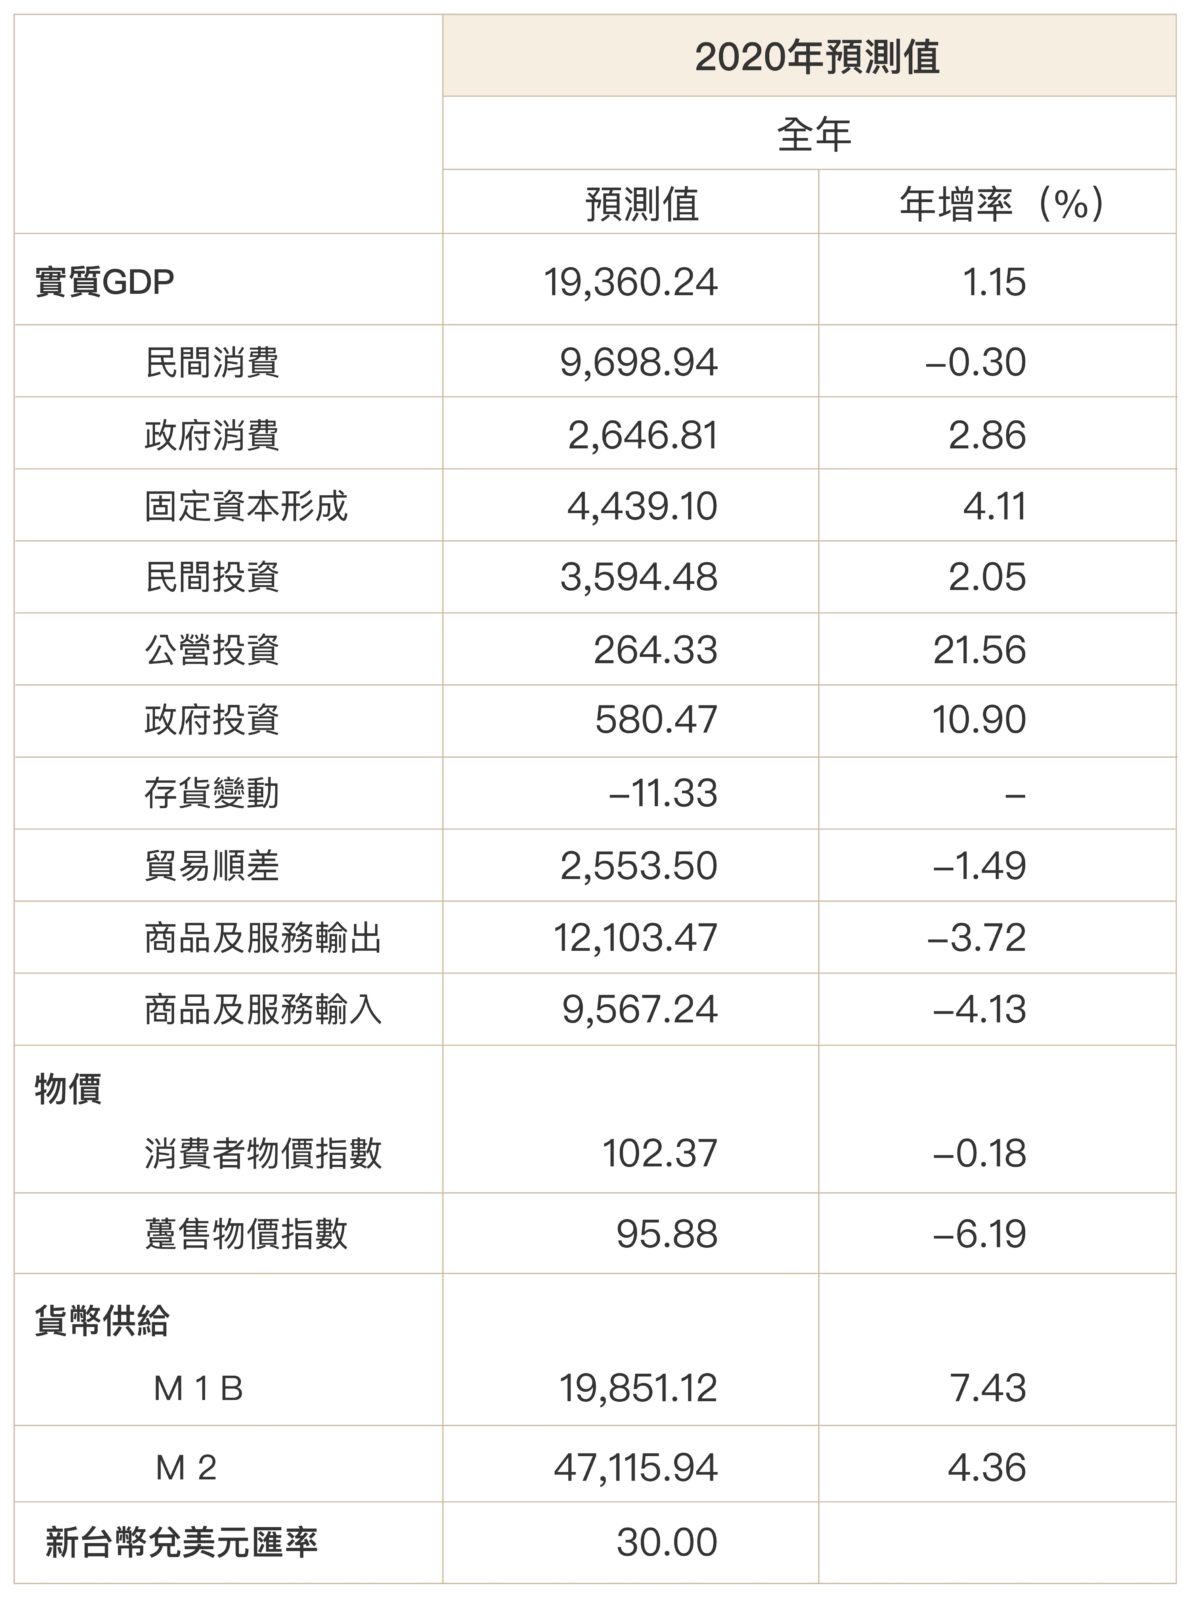
\includegraphics[width=6cm]{pics/predict-demo2.jpeg}
\end{figure}

\end{frame}


\begin{frame}{高维宏观经济数据}
  \begin{itemize}
    \item
    宏观经济指标往往是高维的,难以采用传统模型进行分析。
  \end{itemize}
  \begin{figure}[H]
    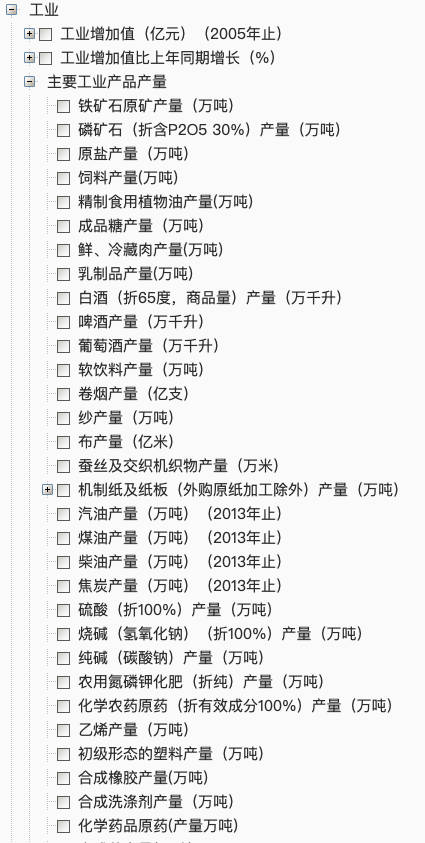
\includegraphics[width=4cm]{pics/var1.png}
    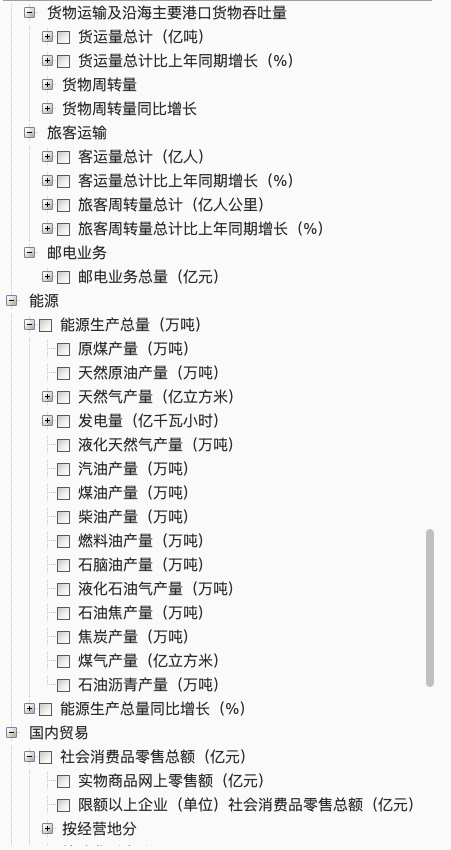
\includegraphics[width=4cm]{pics/var2.png}
  \end{figure}
  
\end{frame}